\documentclass[12pt, a4paper]{report}
\usepackage{graphicx}
\usepackage{amsmath}
\usepackage{float}
\renewcommand{\baselinestretch}{1.2} 
\usepackage{ragged2e}
\usepackage{fancyvrb}
\usepackage{amssymb}
\usepackage[a4paper, total={7in, 9in}]{geometry}
\usepackage[utf8]{inputenc}
\usepackage{physics}
\usepackage{enumitem}


\title{\textbf{EE2703 : Applied Programming Lab \\ Assignment 8 \\ Circuit Analysis using Sympy}} % Title
\author{Arun Krishna A M S \\ EE19B001} % Author name
\date{7th May 2021} % Date for the report

\begin{document}		
		
\maketitle % Insert the title, author and date
\justifying

\section*{Objective}
In this assignment, we try to attain the following objectives: 
\begin{itemize}
  	\item Analysis of Active Filters in laplace domain through \texttt{scipy.signal} toolbox
    \item Explore symbolic algebra capabilities of python using the \texttt{sympy} module
  	\item Analyzing Second order Active Low-pass and High-pass filters by coupling \texttt{sympy} module with \texttt{signal} toolbox
\end{itemize}

\section*{Sympy to Signal class object}
To obtain a time domain output from a \texttt{sympy} transfer function, we must first convert the \texttt{sympy} function into a \texttt{scipy.signal.lti} object. We will then use \texttt{scipy.signal.impulse()} to obtain the time domain function for a given time interval.
The function \texttt{fromSympyToScipy} does this purpose. 

It extracts the expression's numerator and denominator separately into polynomials. The coefficients of these polynomials are then fed into the \texttt{sp.lti} system to get LTI class object with same transfer function \texttt{H}.


\begin{verbatim}
def from_SympyToScipy(H):

    num, denom = sy.fraction(H)
    numerator = sy.poly(num)     
    denominator = sy.poly(denom)   

    numeratorCoeff = numerator.all_coeffs()  
    denominatorCoeff = denominator.all_coeffs()  

    H_SP = sp.lti(p.array(numeratorCoeff, dtype=float), p.array(denominatorCoeff,
    ...dtype=float))

    return H_SP
\end{verbatim}

\clearpage

\section*{Low Pass Filter}
Consider the following active low pass filter circuit
\begin{center}
	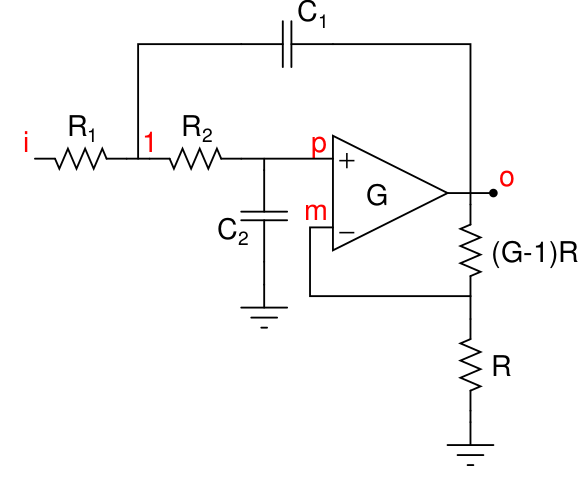
\includegraphics[scale=0.5]{Figure 1.png} 
	\label{fig:rawdata}
\end{center}
where $G = 1.586$ and $R_1 = R_2 = 10k\Omega$ and $C_1 = C_2 = 1nF$. This gives a $3dB$ Butterworth filter with cutoff frequency of $\frac{1}{2\pi} \times 10^5$ Hz. The given circuit is a low pass filter in \textbf{Sallen-Key Topology}. The corresponding equations for the \textbf{Modified Nodal Analysis} circuit are

\begin{equation}
V_m = \frac{V_o}{G}\\
\end{equation}
\begin{equation}
V_p = V_1 \frac{1}{1 + sR_2C_2}\\
\end{equation}
\begin{equation}
V_o = G(V_p - V_m)\\
\end{equation}
\begin{equation}
\frac{V_i - V_1}{R_1} + \frac{V_p - V_1}{R_2} + sC_1(V_o - V_1) = 0
\end{equation}


In matrix format
\begin{equation*}
\begin{pmatrix}
0   & 0 & 1  & -1/G \\
\frac{-1}{sR_2C_2}  & 1 & 0 & 0\\
0  & -G & G & 1 \\
\frac{-1}{R_1} - \frac{1}{R_2} - s*C_1 & \frac{1}{R_2} & 0 & sC_1
\end{pmatrix}
.
\begin{pmatrix}
V_1\\
V_p\\
V_m \\
V_o
\end{pmatrix}
=
\begin{pmatrix}
0 \\
0 \\
0 \\
\frac{-V_i(s)}{R_1} \\
\end{pmatrix}
\end{equation*}

Solving the matrix equation using \texttt{sympy} module and obtaining the transfer function
\begin{verbatim}
def lowPass_filter(R1, R2, C1, C2, G, Vi):
    M = sy.Matrix([[0, 0, 1, -1/G], [-1/(1+R2*C2*s), 1, 0, 0], [0, -G, G, 1], [(1/R1 + 1/R2 +
    ... C1*s), -1/R2, 0, -C1*s]])
    N = sy.Matrix([0, 0, 0, Vi/R1])
    V = M.inv()*N
    return M, N, V

M,N,H = lowPass_filter(10000,10000,1e-9,1e-9,1.586,1)
H = H[3]
\end{verbatim}

After evaluating the values for the frequency response from the symbols using \texttt{lambdify} function, the bode plot of the system is plotted.

\begin{center}
	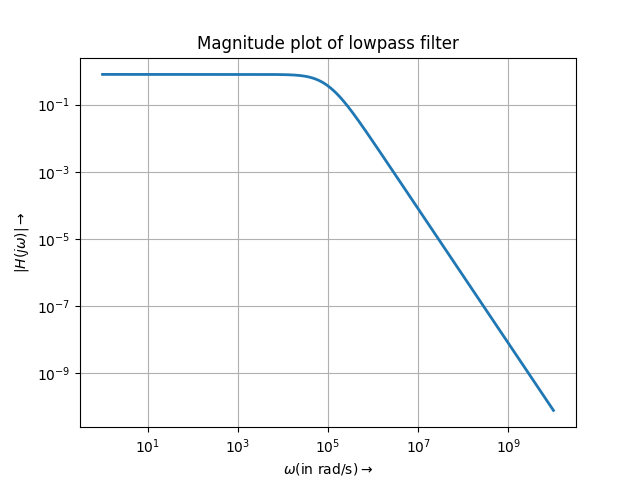
\includegraphics[scale=0.82]{Figure_1.png} 
	\label{fig:rawdata}
\end{center}
As expected the low pass filter has a second order pole at around $10^5$ rad/s.

The output for the stepresponse is obtained by passing the unit step function as input. 
\begin{verbatim}
time = p.linspace(0, 0.001, 1000)
Vout = from_SympyToScipy(H*1/s)
time, stepResponse = sp.impulse(Vout, None, time)
\end{verbatim}

\begin{center}
	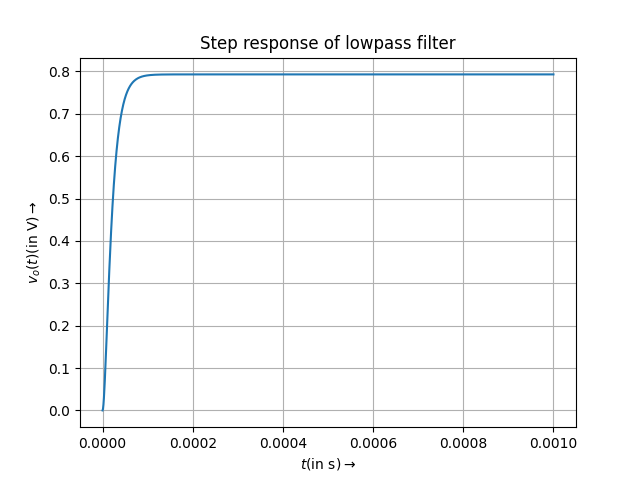
\includegraphics[scale=0.72]{Figure_2.png} 
	\label{fig:rawdata}
\end{center}

The step response of the system steadies with time giving a constant output. This is expected as Lowpass Filters allow DC power to pass through.

Let us try to find an output for an input containing multiple frequencies 
\begin{equation}
v_i(t) = ( sin(2000\pi t) + cos(2 \times 10^6 \pi t))u(t)
\end{equation}

\begin{verbatim}
time = p.linspace(0, 0.01,100000)
Vin = p.sin(2e3*p.pi*time)+p.cos(2e6*p.pi*time)
time, Vout, svec = sp.lsim(from_SympyToScipy(H), Vin, time)
\end{verbatim}

\begin{center}
	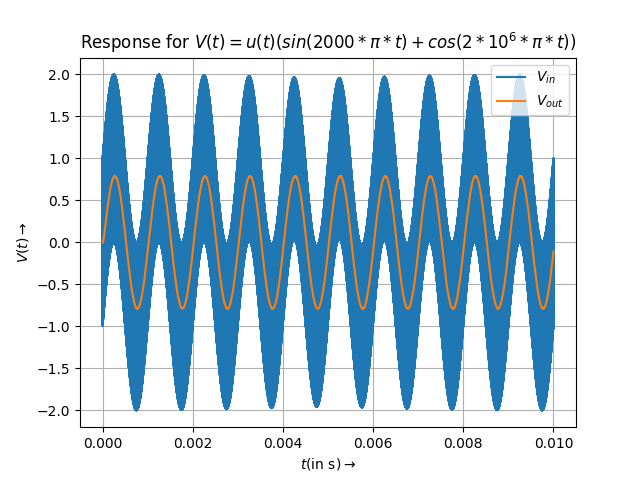
\includegraphics[scale=0.72]{Figure_3png.png} 
	\label{fig:rawdata}
\end{center}

The input signal is a combination of two frequencies, one with low frequency($2000$ rad/s) that lie within the 3dB bandwidth and another with high frequency($2 \times 10^6$ rad/s) that lies outside. The Lowpass Filter attenuatess the high frequency component and the output will only contain the low frequency component.

\section*{High Pass Filter}
Consider the following active high pass filter circuit
\begin{center}
	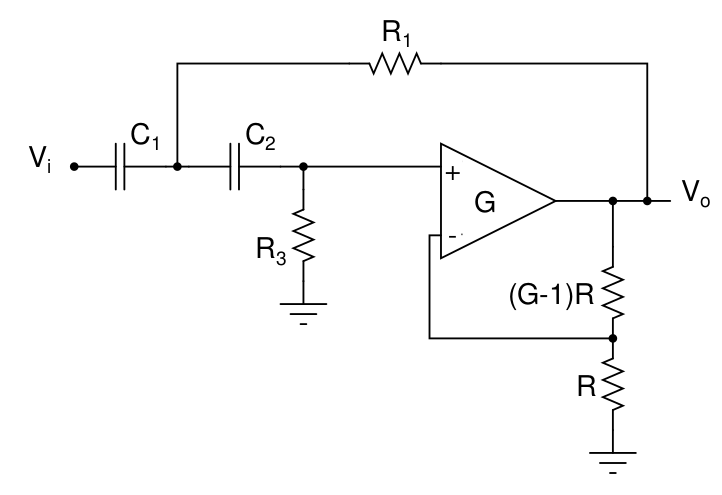
\includegraphics[scale=0.5]{FigureX.png} 
	\label{fig:rawdata}
\end{center}
where $G = 1.586$ and $R_1 = R_3 = 10k\Omega$ and $C_1 = C_2 = 1nF$. This gives a $3dB$ Butterworth filter with cutoff frequency of $\frac{1}{2\pi} \times 10^5$ Hz. The given circuit is a low pass filter in \textbf{Sallen-Key Topology}. The corresponding equations for the \textbf{Modified Nodal Analysis} circuit are

\begin{equation}
V_m = \frac{V_o}{G}\\
\end{equation}
\begin{equation}
V_p = \frac{sC_2R_3V_1}{1 + sR_3C_2}\\
\end{equation}
\begin{equation}
V_o = G(V_p - V_m)\\
\end{equation}
\begin{equation}
V_1(C_1s + C_2s + \frac{1}{R_1}) - sC_1V_i - \frac{V_i}{R_1} - sC_2V_p = 0
\end{equation}
\clearpage
In matrix format
\begin{equation*}
\begin{pmatrix}
0   & 0 & 1  & 1/G \\
-\frac{sC_2R_3}{1+sC_2R_3}  & 1 & 0 & 0\\
0  & -G & G & 1 \\
sC_2 + \frac{1}{R_1} + sC_1 & -sC_2 & 0 & -\frac{1}{R_1}
\end{pmatrix}
.
\begin{pmatrix}
V_1\\
V_p\\
V_m \\
V_o
\end{pmatrix}
=
\begin{pmatrix}
0 \\
0 \\
0 \\
sC_1V_i(s) \\
\end{pmatrix}
\end{equation*}

Solving the matrix equation using \texttt{sympy} module and obtaining the transfer function
\begin{verbatim}
def highPass_filter(R1, R3, C1, C2, G, Vi):

    M = sy.Matrix([[0, 0, 1, -1/G], [-R3*C2*s/(1+R3*C2*s), 1, 0, 0], [0, -G, G, 1], [(C1*s + 
    ... C2*s + 1/R1), -C2*s, 0, -1/R1]])
    N = sy.Matrix([0, 0, 0, Vi*s*C1])
    V = M.inv()*N

    return M, N, V

M,N,H = highPass_filter(10000,10000,1e-9,1e-9,1.586,1)
H = H[3]
\end{verbatim}

After evaluating the values for the frequency response from the symbols using \texttt{lambdify} function, the bode plot of the system is plotted.

\begin{center}
	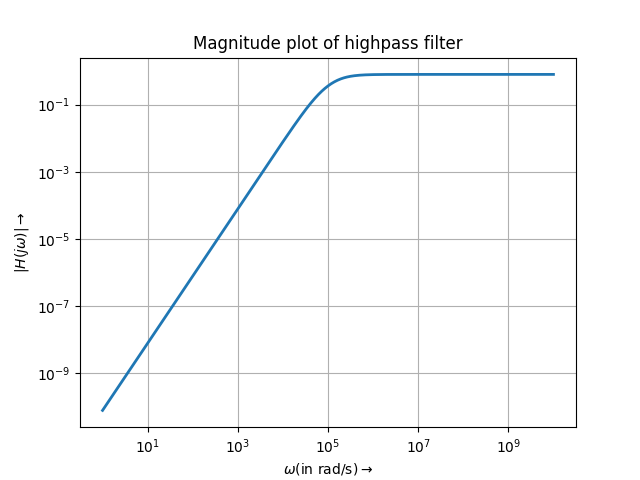
\includegraphics[scale=0.82]{Figure4.png} 
	\label{fig:rawdata}
\end{center}

The output for the stepresponse is obtained by passing the unit step function as input. 
\begin{verbatim}
time = p.linspace(0, 0.001, 1000)
Vout = from_SympyToScipy(H*1/s)
time, stepResponse = sp.impulse(Vout, None, time)
\end{verbatim}

\begin{center}
	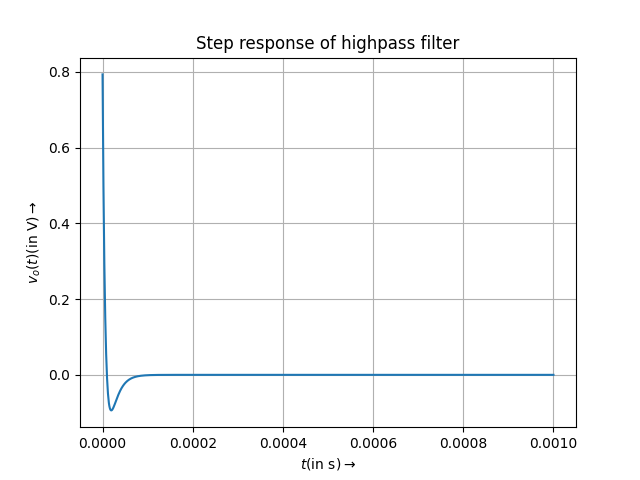
\includegraphics[scale=0.72]{Figure7.png} 
	\label{fig:rawdata}
\end{center}

As expected, the high pass filter attenuates the DC. The reason for the initial peak is the initial conditions. The capacitor does not allow instantaneous changes in the voltage across it. Before t = 0, both capacitors have no charge, and the voltage across both is 0.

The instant the $1V$ is applied $(t = 0+)$, the drop across the capacitors $C_1$ and $C_2$ will still be zero. From equation $6$ and $8$
\begin{equation*}
V_p = V_i\
\end{equation*}
\begin{equation*}
\implies V_o = G(V_i - \frac{V_o}{G})\\
\end{equation*}
\begin{equation*}
\implies V_o = \frac{GV_i}{2} = \frac{1.586}{2} \approx 0.793\\
\end{equation*}
As expected this is shown up in the graph.
\\

When we pass an input with mixed frequencies, only those components which have frequencies above the cutoff can give an output response while the lower frequency components get attenuated.

Let us analyse the output of the system for an input signal of a decaying sinusoid. 
Consider a sinusoid of low frequency $2\pi$rad/s:

\begin{verbatim}
time = p.linspace(0, 0.001, 1000)
Vout = from_SympyToScipy(H*1/s)
time, stepResponse = sp.impulse(Vout, None, time)
\end{verbatim}

\begin{center}
	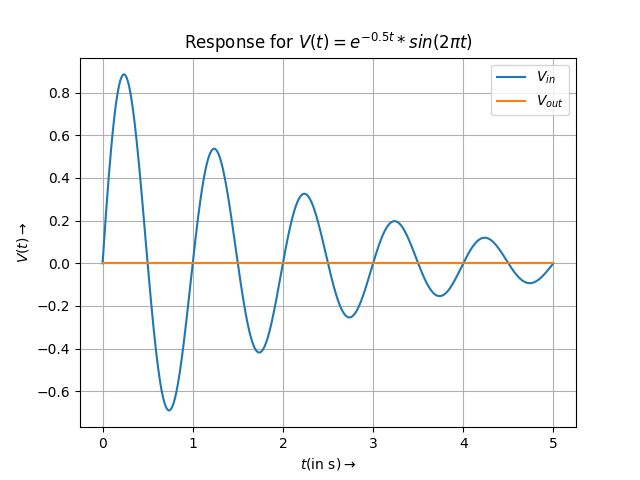
\includegraphics[scale=0.72]{Figure5.png} 
	\label{fig:rawdata}
\end{center}

The system almost completely cuts out this frequency because $2 \pi$rad/s is much lower than $10^5$ rad/s hence the highpass filter shows no output. 

Now let us consider a sinusoid of higher frequency $2\pi \times 10^6$rad/s:

\begin{center}
	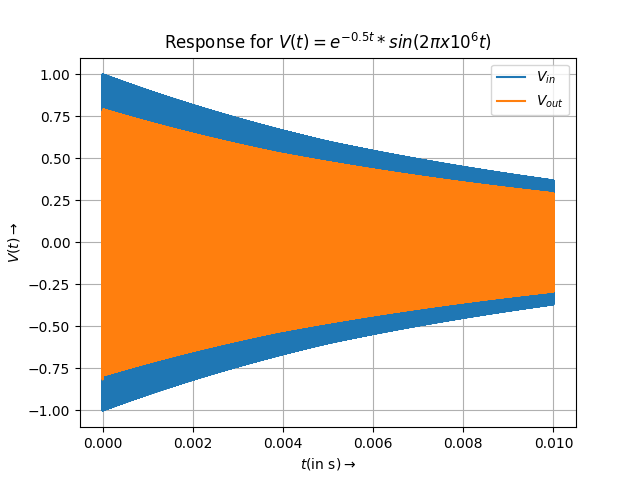
\includegraphics[scale=0.72]{Figure6.png} 
	\label{fig:rawdata}
\end{center}
Since the frequency lies within the pass band, this frequency component gets passed. 

\section*{Conclusion}

Second order Active Lowpass and Highpass filters were analysed using \texttt{sympy} and \texttt{scipy.signal} modules through laplace transform. Bode Plots for both the system were plotted. We also leart to convert the symbolic \texttt{sympy} representation of transfer function to \texttt{scipy} LTI class object after which the processes were performed.  


\end{document}

